%!TEX root = JUrban_SOFT2014.tex

\section{Results} % (fold)
\label{sec:results}

We have selected five time slices from COMPAS shots 4275 and 6962 (i.e. 10 cases in total) for the analysis. These cases include circular, elongated and diverted plasmas with different currents. 

\subsection{Example cases}

A comparison of plasma shapes for shot 4275 is shown in Fig. \ref{fig:ex4275}. Numerical values of reconstruction errors are presented in Table \ref{table:ex4275}. We can observe a very good agreement between the original equilibrium and the reconstructed shapes. In this case, FREEBIE was using linear $p'$ and $FF'$ polynomials so that the EFIT++ model agrees with the target data. VacTH uses 8 magnetic probes and 16 flux loops. As we discuss later, flux loops are essential for reliable VacTH results. Even global kinetic properties are well reconstructed in EFIT++; the largest error around 10~\% is in $l_{\mathrm i}$ (i.e. basically in the toroidal current density profile).

\begin{table*}
\centering

\begin{tabular}{lrrrrrrrrrrrrr}
\toprule
   code &  time &  $\Delta R_{\mathrm in}$ &  $\Delta R_{\mathrm out}$ &  $\Delta Z_{\mathrm min}$ &  $\Delta Z_{\mathrm max}$ &  $\delta \kappa$ &  $E_\mathrm{mp}$ &  $E_\mathrm{fl}$ &  $\delta W$ &  $\delta l_{\mathrm i}$ &  $\delta \beta_{\mathrm p}$ &  $\delta q_0$ &  $\delta q_{95}$ \\
\midrule
 EFIT++ &  0.97 &              0 &            0.002 &        0.001 &        0.001 &                  0.003 &       0.001 &      0.0009 &          0.04 &           0.09 &              0.03 &           0.03 &           0.007 \\
 EFIT++ &  0.99 &          4e-05 &            9e-05 &        0.001 &        0.001 &                  0.004 &       0.001 &      0.0006 &          0.04 &           0.09 &              0.04 &           0.02 &           0.005 \\
 EFIT++ &  1.02 &         0.0005 &           0.0002 &        0.002 &        0.002 &                  0.008 &       0.002 &       0.002 &          0.02 &            0.1 &              0.02 &           0.02 &           0.009 \\
 EFIT++ &  1.05 &          0.001 &           0.0008 &        4e-05 &       0.0003 &                  0.004 &       0.003 &       0.005 &          0.01 &           0.07 &              0.02 &           0.01 &           0.009 \\
 EFIT++ &   1.1 &          0.001 &           0.0005 &        0.005 &       0.0002 &                  0.005 &       0.004 &       0.002 &          0.04 &           0.09 &              0.03 &           0.02 &            0.05 \\
  VacTH &  0.97 &              0 &            0.001 &       0.0006 &       0.0002 &                  0.002 &       8e-07 &       7e-05 &           -- &            -- &               -- &            -- &             -- \\
  VacTH &  0.99 &          4e-05 &           0.0004 &        0.001 &       0.0008 &                  0.004 &       4e-07 &      0.0001 &           -- &            -- &               -- &            -- &             -- \\
  VacTH &  1.02 &          0.002 &           0.0008 &        0.005 &        0.002 &                   0.01 &       2e-06 &       0.002 &           -- &            -- &               -- &            -- &             -- \\
  VacTH &  1.05 &          0.006 &            0.002 &        5e-05 &        0.002 &                   0.01 &       3e-06 &        0.02 &           -- &            -- &               -- &            -- &             -- \\
  VacTH &   1.1 &          0.005 &            0.002 &        0.002 &        0.003 &                   0.02 &       2e-06 &       0.003 &           -- &            -- &               -- &            -- &             -- \\
\bottomrule
\end{tabular}

\caption{Errors for the same cases as in Fig. \ref{fig:ex4275}.}
\label{table:ex4275}
\end{table*}

\begin{figure*}
\centering   %\begin{center}
\hfill{}
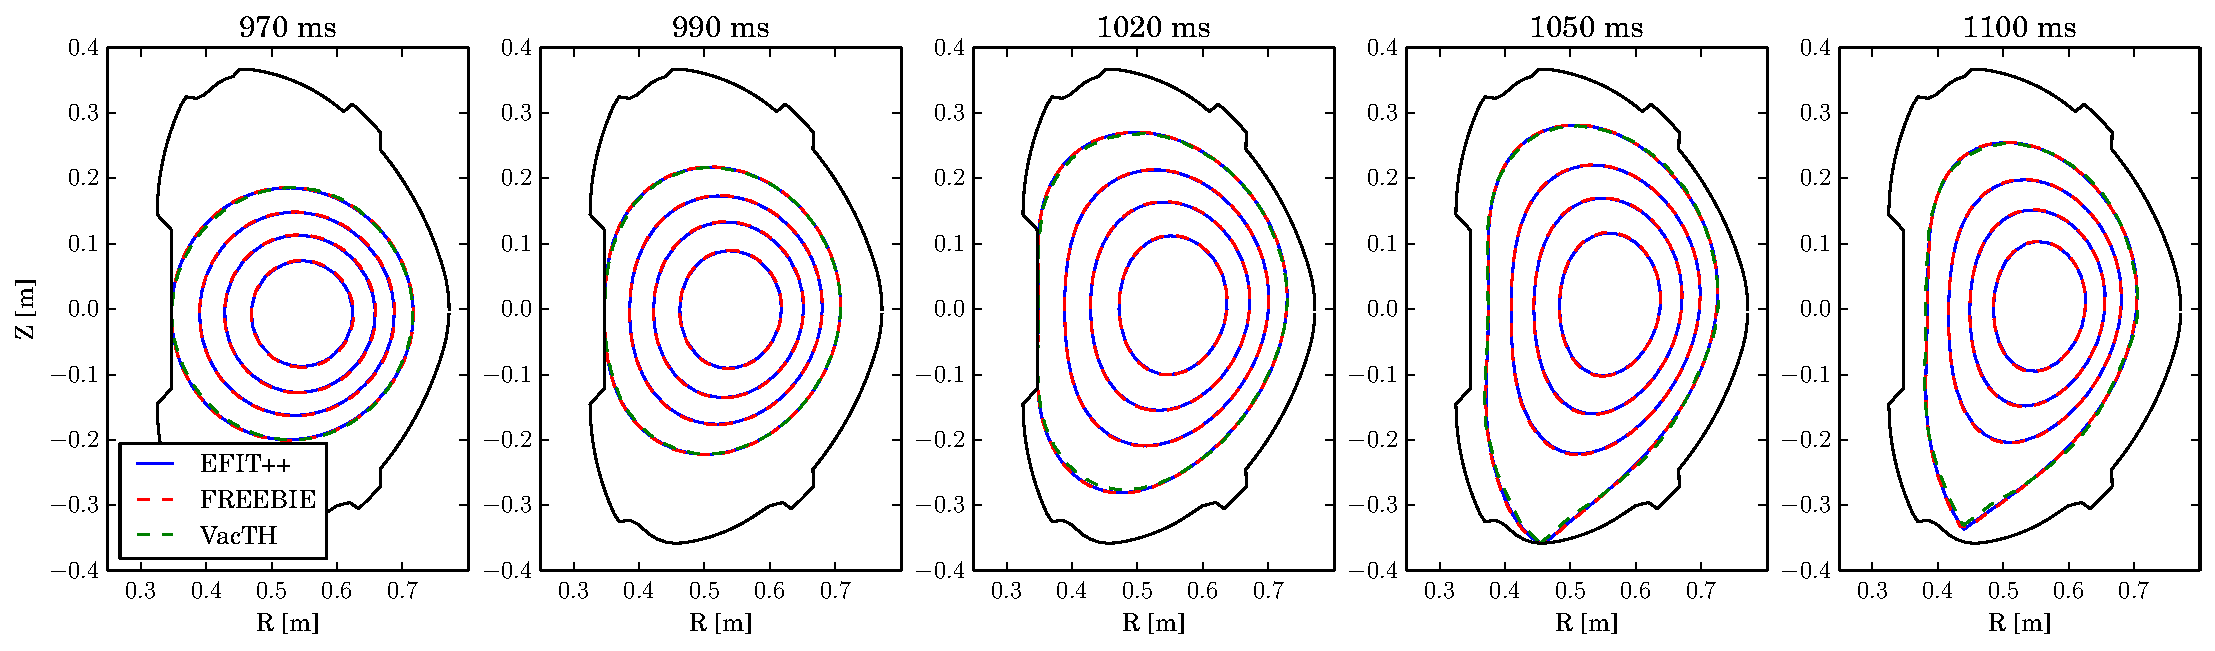
\includegraphics[width=18cm]{figures/example_4275.pdf}
\hfill{}
%\end{center}
\caption{Contours of $\bar\psi=\left(0.25,0.5,0.75,1\right)$, reconstruction from FREEBIE data, shot 4275. EFIT++ parameters: $n_\mathrm{mp} = 16$, $n_\mathrm{fl} = 4$, $n_{p'} = n_{FF'} = 1$. VacTH parameters: $n_\mathrm{mp} = 8$, $n_\mathrm{fl} = 16$, $n_P = n_Q = 5$. $E_\mathrm{mp, fl}$ is the relative error of the reconstructed magnetic probes and flux loops values, respectively.}
\label{fig:ex4275}
\end{figure*}


The second shot for the comparison is 6962, which has been chosen because Thomson scattering (TS) profiles are available. In Fig. \ref{fig:ex6962} we show reconstructions for more realistic equilibria and an artificial noise in the synthetic diagnostic signals. TS pressures were used in FREEBIE equilibria, which course no longer feature linear $p'$ and $FF'$ profiles. 
It is apparent that the reconstruction is not as good as in the previous case. Nevertheless, the plasma shape is well reconstructed with EFIT++ and VacTH, except for the last time slice in which VacTH yields too large plasma in the upper part.
$n_{\mathrm p} = n_{\mathrm q} = 4$ is used in this case as these values are minimum for reasonable VacTH results, while higher values are too sensitive to the input noise.
Expectedly, EFIT++ reconstruction with magnetic data only cannot reliably reconstruct kinetic plasma parameters, such as the stored energy or $q_0$. Rather unexpected is a relatively good agreement of $l_\mathrm{i}$. However, this agreement is compensated by a large error of $\beta_{\mathrm p}$ so that the quantity $\beta_{\mathrm p} + l_{\mathrm i}/2$ remain within a 10~\% error bar. Notable are large errors (up to 40~\%) in the stored energy, even for the circular plasma, which are mainly caused by incompatible pressure profiles.

\begin{figure*}
\centering   %\begin{center}
\hfill{}
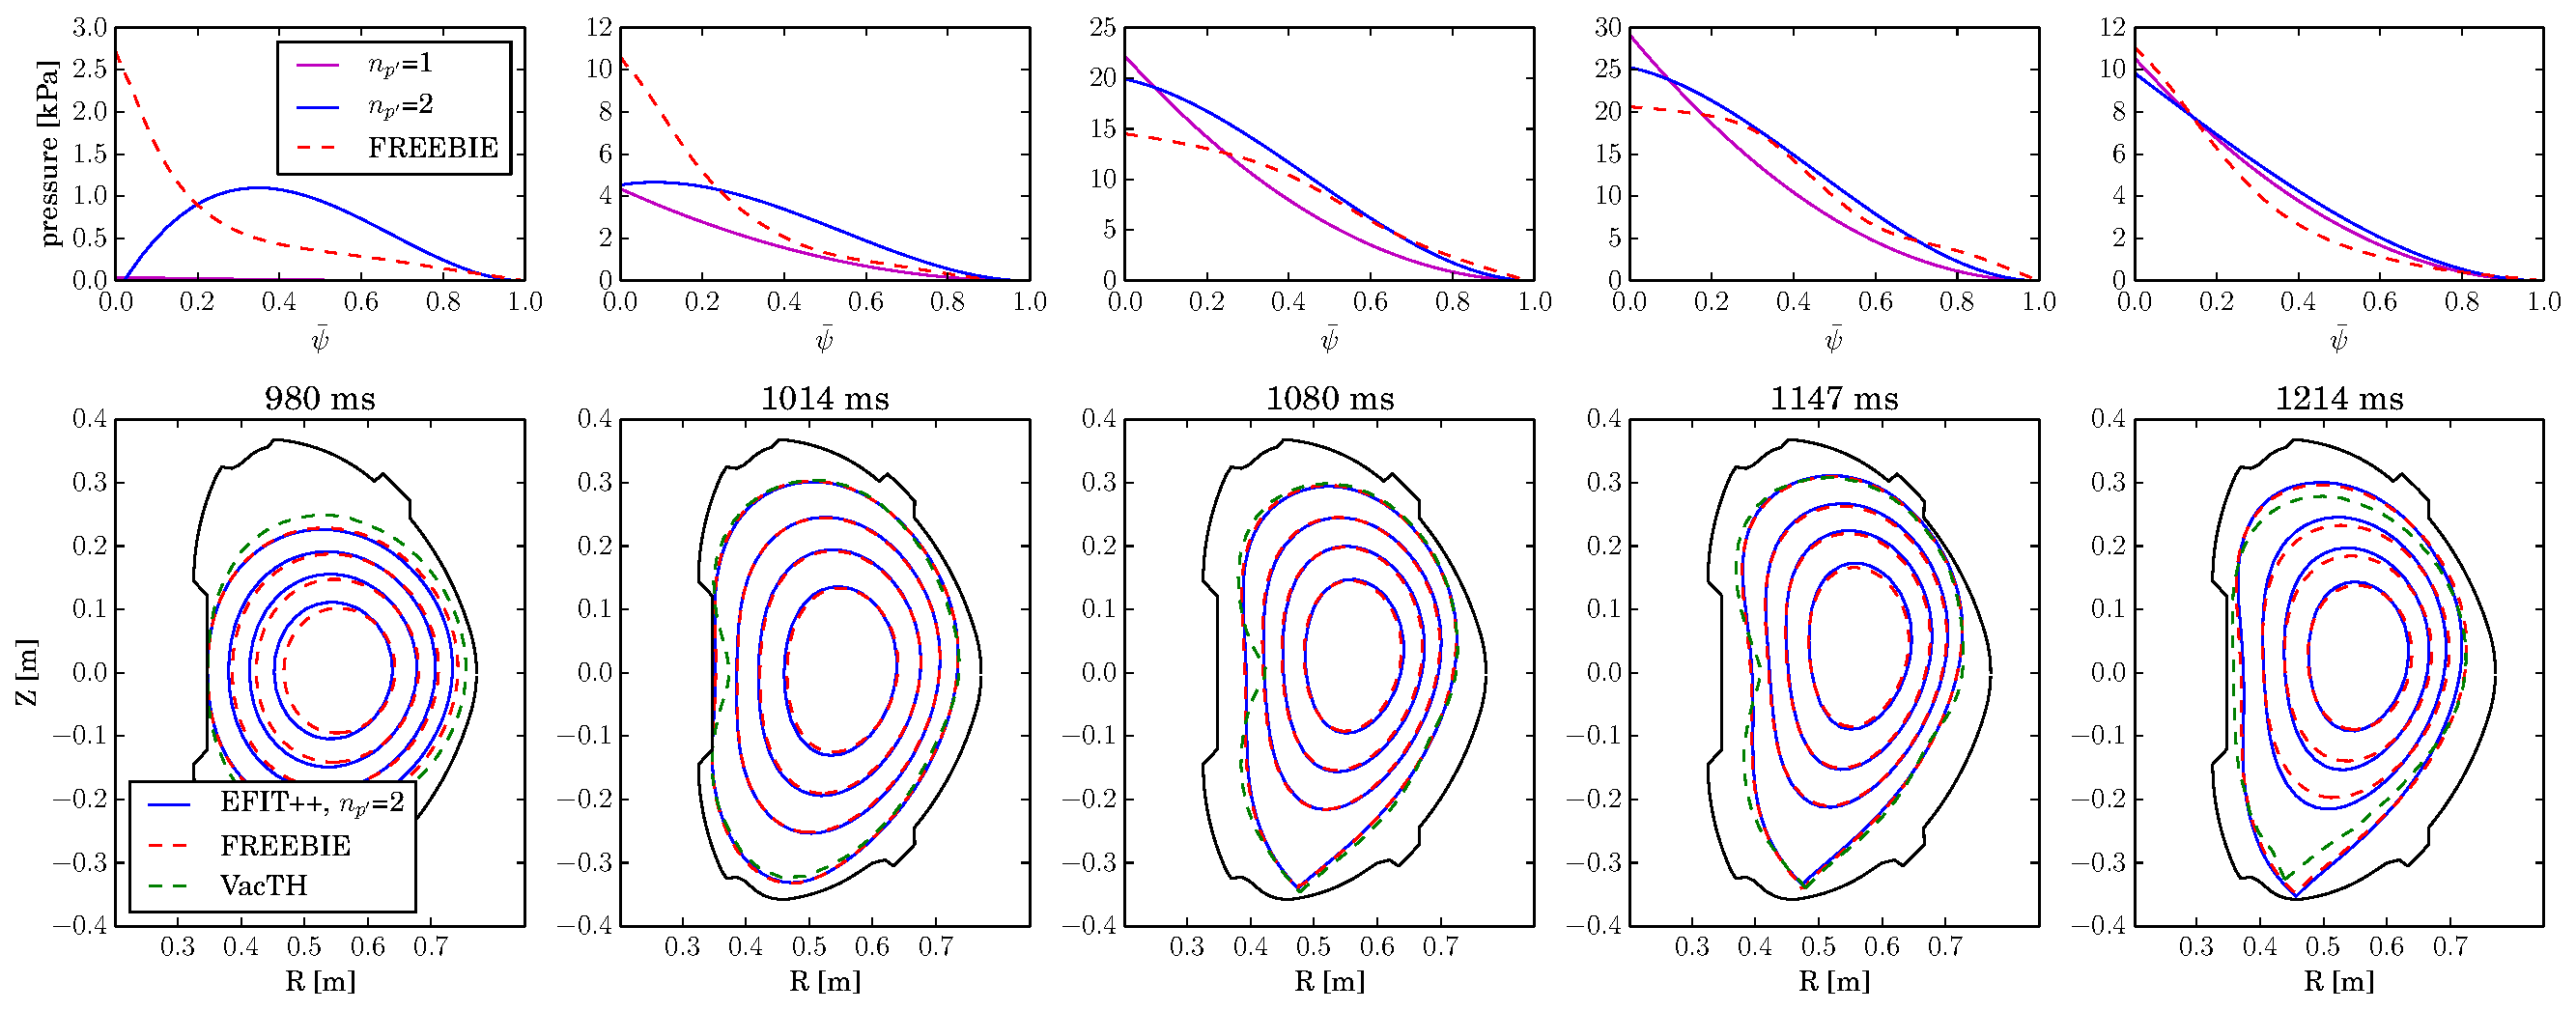
\includegraphics[width=18cm]{figures/example_6962_TS_noise.pdf}
\hfill{}
%\end{center}
\caption{Pressure profiles and contours of $\bar\psi=\left(0.25,0.5,0.75,1\right)$, reconstruction from FREEBIE data, shot 6962 with Thomson scattering pressure profiles. EFIT++ parameters: $n_\mathrm{mp} = 16$, $n_\mathrm{fl} = 4$, $n_{p'} = n_{FF'} = 1$. VacTH parameters: $n_\mathrm{mp} = 8$, $n_\mathrm{fl} = 16$, $n_P = n_Q = 4$.}
\label{fig:ex6962}
\end{figure*}

\begin{table*}
\centering

\begin{tabular}{lrrrrrrrrrrrrr}
\toprule
   % code &  time &  $\Delta R_{\mathrm in}$ &  $\Delta R_{\mathrm out}$ &  $\Delta Z_{\mathrm min}$ &  $\Delta Z_{\mathrm max}$ &  $\delta \kappa$ &  $E_\mathrm{mp}$ &  $E_\mathrm{fl}$ &  $\delta W$ &  $\delta \left(\beta_{\mathrm p} + l_{\mathrm i}/2 \right)$  &  $\delta q_0$ &  $\delta q_{95}$ \\
   code &  time &  $\Delta R_{\mathrm in}$ &  $\Delta R_{\mathrm out}$ &  $\Delta Z_{\mathrm min}$ &  $\Delta Z_{\mathrm max}$ &  $\delta \kappa$ &  $E_\mathrm{mp}$ &  $E_\mathrm{fl}$ &  $\delta W$ &  $\delta l_{\mathrm i}$ &  $\delta \beta_{\mathrm p}$ &  $\delta q_0$ &  $\delta q_{95}$ \\
\midrule
 EFIT++ &  980 &               0 &            0.005 &        0.001 &        8e-06 &                   0.01 &        0.01 &        0.01 &           0.4 &           0.03 &               0.4 &            0.2 &          0.0008 \\
 EFIT++ & 1014 &           0.003 &            0.006 &         0.02 &         0.01 &                   0.06 &        0.03 &        0.03 &           0.3 &          0.008 &               0.3 &            0.2 &            0.08 \\
 EFIT++ & 1080 &           0.007 &            0.002 &        0.005 &        0.002 &                   0.04 &        0.03 &        0.03 &           0.3 &           0.01 &               0.3 &            0.2 &            0.02 \\
 EFIT++ & 1147 &           0.008 &            0.008 &         0.01 &        0.006 &                   0.06 &        0.03 &        0.02 &           0.3 &           0.06 &               0.3 &            0.3 &            0.05 \\
 EFIT++ & 1214 &          0.0002 &            0.008 &        0.002 &        0.001 &                   0.02 &        0.02 &        0.01 &          0.04 &            0.2 &              0.06 &            0.1 &            0.01 \\
  VacTH &  980 &               0 &             0.01 &         0.01 &        0.007 &                   0.02 &      0.0001 &        0.01 &           -- &            -- &               -- &            -- &             -- \\
  VacTH & 1014 &           0.006 &           0.0002 &         0.01 &        0.007 &                   0.03 &       3e-05 &        0.01 &           -- &            -- &               -- &            -- &             -- \\
  VacTH & 1080 &           0.009 &           0.0007 &        0.003 &       0.0007 &                   0.02 &       3e-05 &        0.01 &           -- &            -- &               -- &            -- &             -- \\
  VacTH & 1147 &            0.02 &            0.007 &       0.0009 &        0.002 &                   0.01 &       5e-05 &        0.01 &           -- &            -- &               -- &            -- &             -- \\
  VacTH & 1214 &            0.03 &            0.009 &         0.02 &         0.03 &                   0.02 &      0.0002 &        0.02 &           -- &            -- &               -- &            -- &             -- \\

 % EFIT++ & 1e+03 &               0 &            0.005 &        0.001 &        8e-06 &                   0.01 &        0.01 &        0.01 &           0.4 &           0.03 &               0.4 &            0.2 &          0.0008 \\
 % EFIT++ & 1e+03 &           0.003 &            0.006 &         0.02 &         0.01 &                   0.06 &        0.03 &        0.03 &           0.3 &          0.008 &               0.3 &            0.2 &            0.08 \\
 % EFIT++ & 1e+03 &           0.007 &            0.002 &        0.005 &        0.002 &                   0.04 &        0.03 &        0.03 &           0.3 &           0.01 &               0.3 &            0.2 &            0.02 \\
 % EFIT++ & 1e+03 &           0.008 &            0.008 &         0.01 &        0.006 &                   0.06 &        0.03 &        0.02 &           0.3 &           0.06 &               0.3 &            0.3 &            0.05 \\
 % EFIT++ & 1e+03 &          0.0002 &            0.008 &        0.002 &        0.001 &                   0.02 &        0.02 &        0.01 &          0.04 &            0.2 &              0.06 &            0.1 &            0.01 \\
 %  VacTH & 1e+03 &               0 &             0.01 &         0.01 &        0.007 &                   0.02 &      0.0001 &        0.01 &           -- &            -- &               -- &            -- &             -- \\
 %  VacTH & 1e+03 &           0.006 &           0.0002 &         0.01 &        0.007 &                   0.03 &       3e-05 &        0.01 &           -- &            -- &               -- &            -- &             -- \\
 %  VacTH & 1e+03 &           0.009 &           0.0007 &        0.003 &       0.0007 &                   0.02 &       3e-05 &        0.01 &           -- &            -- &               -- &            -- &             -- \\
 %  VacTH & 1e+03 &            0.02 &            0.007 &       0.0009 &        0.002 &                   0.01 &       5e-05 &        0.01 &           -- &            -- &               -- &            -- &             -- \\
 %  VacTH & 1e+03 &            0.03 &            0.009 &         0.02 &         0.03 &                   0.02 &      0.0002 &        0.02 &           -- &            -- &               -- &            -- &             -- \\

\bottomrule
\end{tabular}
\caption{Errors for the same cases as in Fig. \ref{fig:ex6962}.}
\label{table:ex6962}
\end{table*}


\begin{figure*}
\centering   %\begin{center}
\hfill{}
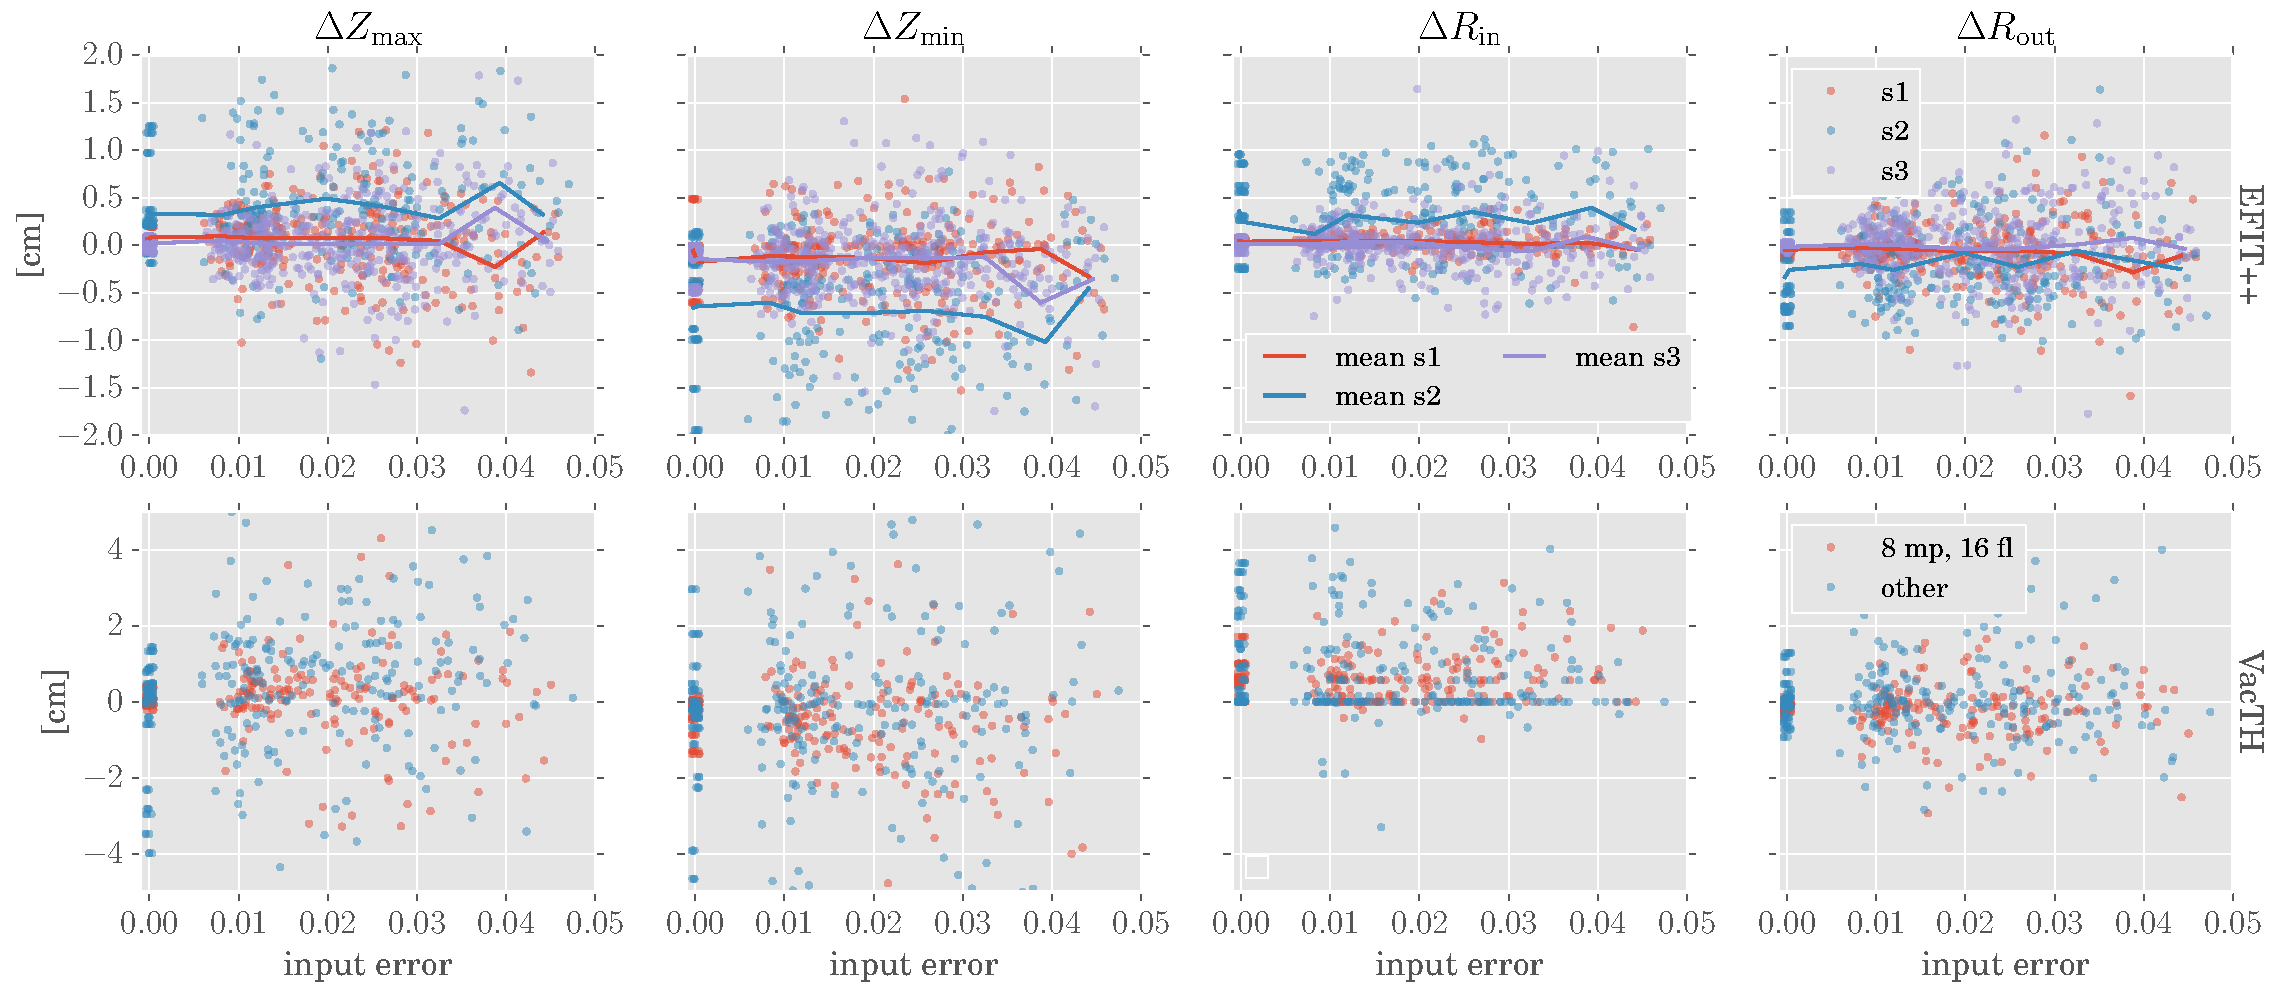
\includegraphics[width=18cm]{figures/RZstats.pdf}
\hfill{}
%\end{center}
\caption{Absolute errors in LCFS extents for convergent cases. EFIT++ results in the first row, VacTH in the second row. Selection 1 means linear $p'$ and $FF'$ in EFIT++ as well as FREEBIE, selection 2 means TS pressure profiles in FREEBIE and $n_{p'} = n_{FF'} = 1$ in EFIT++, selection 3 means TS pressure profiles in FREEBIE and $n_{p'} = 2$ in EFIT++. Input error is calculated as an average of $I_{\rm{p}}$, magnetic probes and flux loops values. Zero input error data are scattered for a better visibility.}
\label{fig:RZstats}
\end{figure*}

\begin{figure*}
\centering   %\begin{center}
\hfill{}
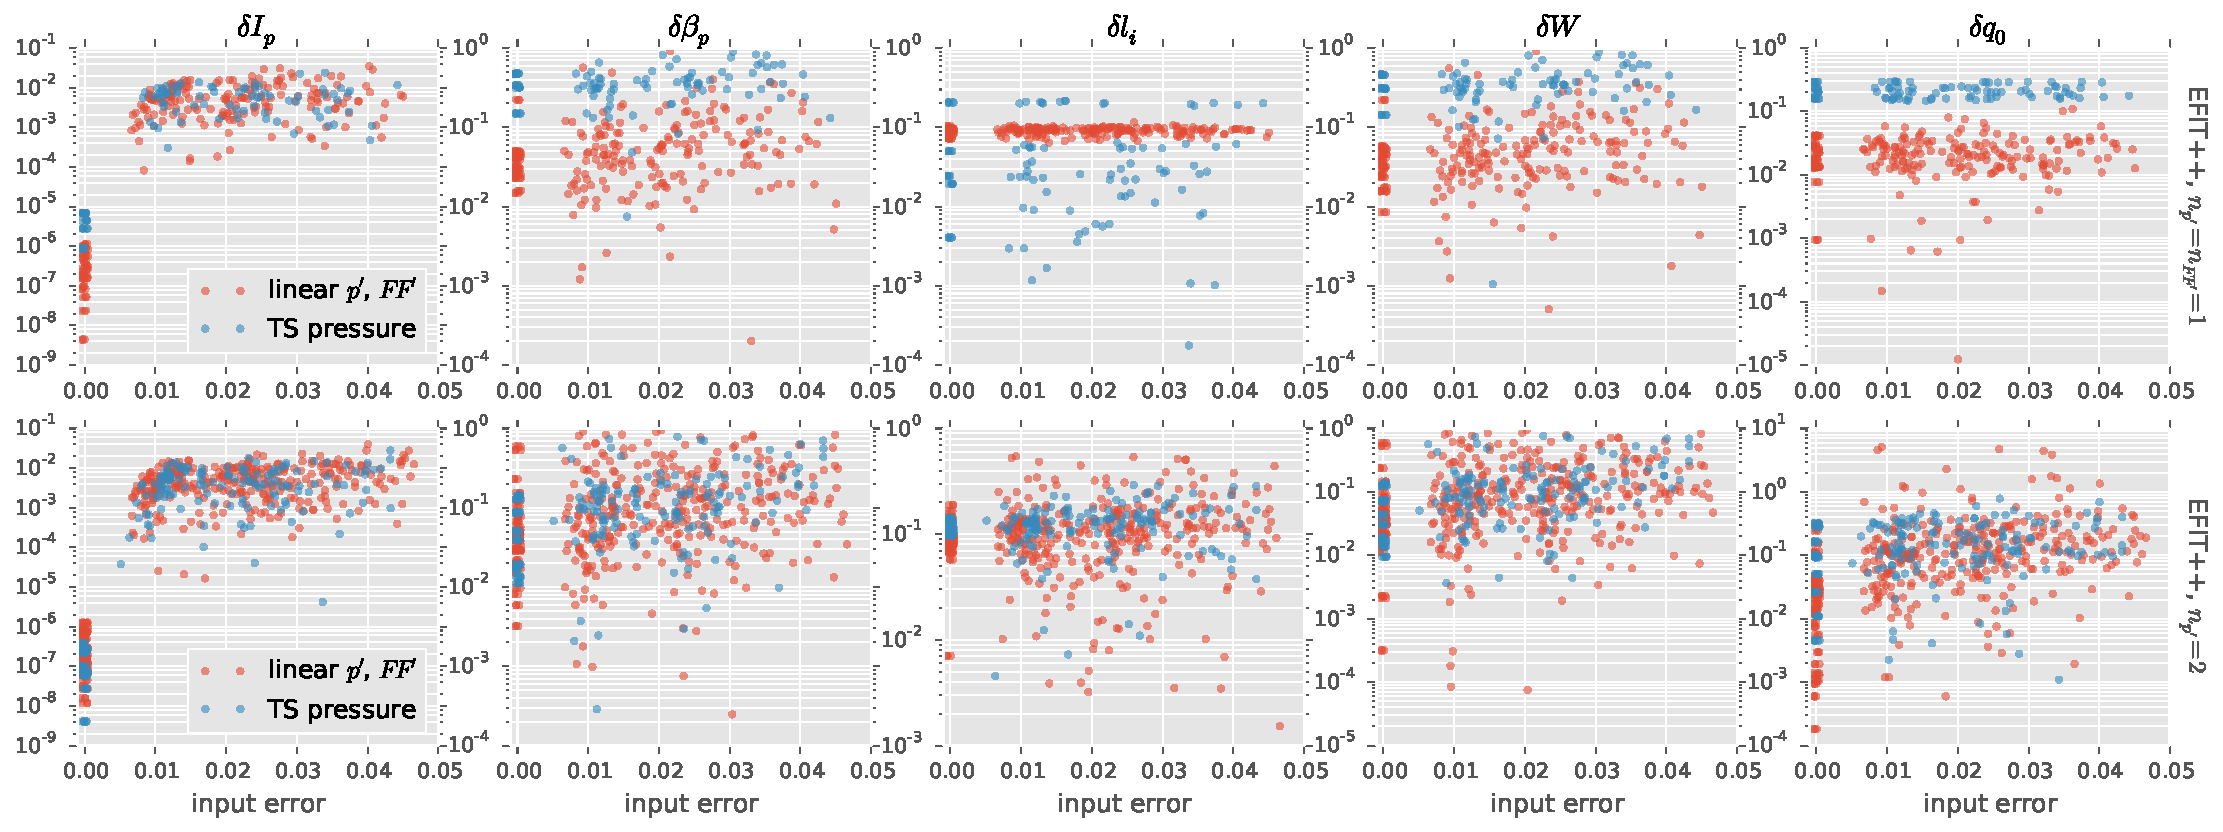
\includegraphics[width=18cm]{figures/kinetic_stats.pdf}
\hfill{}
%\end{center}
\caption{First row: $n_{p'}=n_{FF'}=1$, second row: either $n_{p'}=2$ or $n_{FF'}=2$. Red: linear $p'$ and $FF'$ profiles, blue: TS pressure profiles. Zero input error data are scattered for a better visibility.}
\label{fig:kinetic_stats}
\end{figure*}


\subsection{Statistical analysis} % (fold)
\label{sub:statistical_analysis}

In order to get a global overview of EFIT++ and VacTH reconstruction properties on COMPASS, we perform a scan over major code parameters and signal noise levels. In particular, $n_{p',FF'} = 1,2 $, $(n_\mathrm{mp}, n_\mathrm{fl}) = (16, 4), (64, 4), (8, 16)$, $\epsilon = 0, 0.02, 0.04, 0.06$, $n_{P,Q} = 4, 5, 6$. The same cases as above (time slices of shots 4275 and 6962) are used as target equilibria. For shot 6962, equilibria with TS pressure profiles and with linear $p'$ and $FF'$. This means there is 15 different target equilibria in total.

Absolute errors of the reconstructed LCFS extents for convergent cases from the scan are shown in Fig. \ref{fig:RZstats}. We can observer that the LCFS reconstructed with EFIT++ for target linear $p'$ and $FF'$ profiles (selection 1) are within 1~cm errors. There are, however, cases with up to 3 cm errors in $Z_{\rm{min}}$ for the more realistic TS pressure profiles (selection 2) if $n_{p'}=1$ is used. This error can be reduced by using $n_{p'}=2$. Input errors do not pose major difficulties for EFIT++. 

VacTH is performing reasonably well for its most favourable diagnostic set of 8 magnetic probes and 16 flux loops and $n_P = n_Q = 4$. With a higher number of harmonics or with less flux loops, VacTH becomes unreliable and yields significant errors. Unfortunately, only 4 flux loops are currently available on COMPASS. In fact, it is easier for VacTH to fit magnetic probes than flux loops while magnetic probes do not fully determine the magnetic flux. This is also apparent in $E_\mathrm{mp}$ and $E_\mathrm{fl}$ values in Tables \ref{table:ex4275} and \ref{table:ex6962}. An additional optimization of the fitting weights or algorithm is probably needed. This can be demonstrated by an exercise reconstruction with 64 magnetic probes and 16 flux loops, whose result is significantly worse than with only 8 magnetic probes and 16 flux loops.

EFIT++ internal plasma parameters reconstruction results are shown in Fig. \ref{fig:kinetic_stats}. 


Failure rates ...

% subsection statistical_analysis (end)



% section results (end)
